\documentclass[a4paper]{report}

% \usepackage{a4wide}
\usepackage{graphicx}
\usepackage{wrapfig}
\usepackage[utf8]{inputenc}
\usepackage{blindtext}
\usepackage{amsmath}
\usepackage{amssymb}
\usepackage{amsfonts}
\usepackage{physics}
\usepackage{setspace}
\usepackage{mathrsfs}

\onehalfspacing

\newcommand{\problem}[1]{$\vb*{\mathsection}$ \textbf{Problema #1.}}
\newcommand{\letter}[1]{\vspace*{3mm}\textbf{(#1)} \hspace{1mm} }
\newcommand{\levicivita}[1]{\epsilon_{#1}}

\usepackage{accents}
\newcommand*{\dt}[1]{%
  \accentset{\mbox{\large\bfseries .}}{#1}}
\newcommand*{\ddt}[1]{%
  \accentset{\mbox{\large\bfseries .\hspace{-0.25ex}.}}{#1}}
\newcommand*{\dddt}[1]{%
  \accentset{\mbox{\large\bfseries .\hspace{-0.25ex}.\hspace{-.20ex}}}{#1}}
\newcommand*{\dnt}[2][4]{\dt{#2}^{\tiny(#1)}}


\newcommand{\listnumber}[1]{
  \begin{center}
    \Large
    \textbf{FIS 108 Eletrodinâmica Clássica I - Lista #1} \\
    \large
    Alex Enrique Crispim
    \normalsize
  \end{center}
}

\newcommand{\statment}[1]{\textit{#1} \vspace*{5mm}}
\newcommand{\aspas}[1]{``#1''}


\begin{document}
\listnumber{1}

\problem{1} \textit{Use Gauss's theorem (and (1.21) if necessary) to prove the following:}

\letter{a} \textit{Any excess charge placed on a conductor must lie on its surface. (A conductor, by definition, contains charges capable of moving freely under the action of applied electric fields.)}

Comecemos provando o Teorema de Earnshaw para argumentar que o campo elétrico no interior de um condutor deve ser nulo.

Suponha que tenha-se uma carga em uma região onde existe um campo elétrico $\vb{E} = -\grad{\Phi}$. Vamos supor que exista um ponto $P$, que não esteja na fronteira do espaço onde tem-se o campo elétrico, tal que $\Phi$ assuma um valor mínimo. Então, ao se afastar de $P$ tem-se um aumento no potencial, para qualquer direção. Podemos escrever esse fato como
\begin{equation*}
  \pdv{\Phi}{\vb{n}^\prime} = \grad{\Phi} \vdot \vu{n}^\prime > 0
  \quad \forall \vb{n}^\prime .
\end{equation*}
Tomando uma superfície fechada $S$ próxima do ponto $P$, englobando o mesmo, temos que
\begin{equation*}
  \oint_S \pdv{\Phi}{\vb{n}^\prime} \dd{a} > 0.
\end{equation*}
Por outro lado, a lei de Gauss nos fornece
\begin{equation*}
  \oint_S \pdv{\Phi}{\vb{n}^\prime} \dd{a} = \int_V \laplacian{\Phi} \dd[3]{x} = 0
\end{equation*}
contradizendo o resultado anterior. Analogamente, temos para o caso onde $P$ é um máximo do potencial.

Como consequência, temos que \textit{o potencial eletrostático só pode assumir um valor mínimo ou máximo no bordo da região onde tem-se um campo elétrico}.

Do teorema anterior, vê-se que uma carga elétrica, $q$, não pode estar em equilíbrio em uma região onde há campo elétrico, pois sua energia potencial $q\Phi$ não apresenta um mínimo, senão na borda do espaço. Assim, nenhuma configuração de cargas pode ser estável apenas por interações eletrostáticas.

Do resultado acima, se tivermos cargas no interior de um condutor, haverá um campo elétrico resultante (o que se pode ver facilmente pela lei de Gauss), levando a um potencial eletrostático, consequentemente. Como tal configuração de cargas não é estável, as mesmas tendem a ir para o bordo do espaço em questão, isto é, para a superfície do material. É claro que o bordo deve representar um mínimo do potencial, neste caso, pois se fosse um máximo, as cargas não poderiam ir para tal região, caindo no problema anterior.

Segue, portanto, que o campo elétrico no interior de um condutor deve se anular, no caso estacionário.

Um outro modo de ver este problema envolve um argumento diferente: no caso estacionário não podem haver correntes no interior do condutor, pois o movimento de correntes leva a dissipação de energia, portanto, não pode existir sem um agente externo realizando trabalho. Com isso, $\vb{E}^{(int)} = 0$.

Para mostrar que as cargas devem se distribuir na superfície do condutor, usamos a ideia desenvolvida pode Lorentz (1902) de que os campos macroscópicos podem ser obtidas tomando-se a média para os campos microscópicos. Seja $\vb{e}$ o campo elétrico microscópico, temos
\begin{equation*}
  0 = \div{\vb{E}^{(int)}} = \div{\ev{\vb{e}}} = \ev{\rho} / \epsilon_0 \Leftrightarrow \ev{\rho} = 0,
\end{equation*}
com $\rho$ sendo a densidade miscroscópica de cargas. Para anular a densidade de carga no interior, as cargas devem estar distribuidar na superfície do condutor.

\letter{b}
\textit{A clossed, hollow condutor shields its interior from fields due to charges outside, but does not shield its exterior from the fields due to charges placed inside it.}

No interior do condutor, quando não existem cargas, a Lei de Gauss fornece
\begin{equation*}
  \oint_S \vb{E} \vdot \dd{\vb{a}} = 0,
\end{equation*}
para toda superfície $S$ fechada no interior do condutor. Logo, o campo elétrico no interior deve se anular;
\begin{equation*}
  \vb{E} = 0 \quad \text{(inteior).}
\end{equation*}

Por outro lado, se existe uma carga total $q$ no interior do condutor, para uma superfície $S$ externa ao condutor, englobando o mesmo, é fácil ver que
\begin{equation*}
  \oint_S \vb{E}\vdot \dd{\vb{a}} \neq 0,
\end{equation*}
seja qual for $S$. Como existe sempre um fluxo do campo sobre a superfície, o mesmo é não nulo. Está mostrado o resultado.

\letter{c}
\textit{The electric field at the surface of a conductor is normal to the surface and has a magnitude $\sigma/\epsilon_0$, where $\sigma$ is the charge density per unit area on the surface.}

Vamos considerar a direção $z$ como sendo normal a um ponto arbitrário da superfície do condutor e olhar para o entorno desse. Lembrando que $\curl{\vb{E}} = 0$, temos o seguinte:

Podemos utilizar que
\begin{equation*}
  \oint \vb{E} \vdot \dd{\vb{l}} = 0
\end{equation*}
para deduzir uma condição de contorno para o campo elétrico ao atravessar a interface (superfície do condutor) que separa o meio interno do meio externo. Considere a figura abaixo:

\begin{figure}[h]
  \center
  \includegraphics[scale = .27]{./imgs/matching_conditions.png}
  \caption{Diagrama de uma região infinitesimal de uma superfície de separação entre dois meios (meios 1 e 2, da figura). $\Gamma$ é um caminho retangular fechado que contém partes em ambos os meios. $a$ e $b$ são as medidas dos lados do caminho. O caminho $\Gamma$ é composto pela união dos caminhos $\gamma_j$ (j = 1,...,4), que descrevem cada lado. $\vu{l}_i$ ($i$ = 1,3) denotam os versores diretores das curvas $\gamma_i$.}
\end{figure}

Podemos escrever
\begin{equation*}
  0 = \oint \vb{E} \vdot \dd{\vb{l}} = \int_{\gamma_1} \vb{E} \vdot \dd{\vb{l}} + \int_{\gamma_2} \vb{E} \vdot \dd{\vb{l}} + \int_{\gamma_3} \vb{E} \vdot \dd{\vb{l}} + \int_{\gamma_4} \vb{E} \vdot \dd{\vb{l}}.
\end{equation*}
No limite $a \to 0$, as os caminhos $\gamma_{2,4}$ passam a não contribuir para a integral de modo que
\begin{equation*}
  \int_{\gamma_1} \vb{E} \vdot \dd{\vb{l}} + \int_{\gamma_3} \vb{E} \vdot \dd{\vb{l}} \sim 0, \quad \text{quando } a \to 0.
\end{equation*}
Considerando os versores diretores das curvas $\gamma_{1,3}$, $\vu{l}_{1,3}$, da figura, podemos calcular a integral acima sob a hipótese de que o comprimento $b$ seja muito pequeno de tal forma que o campo seja aproximadamente uniforme. Com isso,
\begin{equation*}
  \int_{\gamma_i} \vb{E}_i \vdot \dd{\vb{l}} = b \vb{E} \vdot \vu{l}_i,
\end{equation*}
Onde $\vb{E}_i$ denota o campo elétrico no meio ``$i$''.
Observando que $\vu{l}_1 = - \vu{l}_3$, podemos escrever a soma das integrais anteriores como
\begin{equation*}
  (\vb{E}_1 - \vb{E}_3) \vdot \vu{l}_1 = 0,
\end{equation*}
onde eliminamos o fator $b$, irrelevante. Notando que $\vb{E}_i \vdot \vb{l}_i$ é o campo tangencial, podemos finalmente entender a condição de contorno acima como: ``\textit{a componente tangencial do campo elétrico é constante através da interface que separa dois meios}''.

Para o caso específico de um condutor, como o campo interno é nulo, segue que a componente tangencial do campo elétrico deve se anular. Assim, o campo é normal à superfície do condutor (Figura 2 abaixo). Um outro fato importante que segue é que a superfície de um condutor é uma equipotencial. Isso segue da expressão $\vb{E} = - \grad{\Phi}$.

\begin{figure}[h]
  \center
  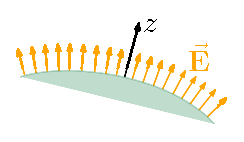
\includegraphics[scale = 1.1]{./imgs/surf.eps}
  \caption{Campo elétrico nas imediações de um condutor. O campo é normal à superfície; as linhas de campo emergem ou terminam na superfície do condutor.}
\end{figure}

Com as informações obtidas, podemos utilizar a Lei de Gauss para obter o campo elétrico na vizinhança do condutor.

Seja $\sigma$ a densidade superficial de carga no condutor, considere uma superfície $S_g$ como a representada na figura abaixo.

\begin{figure}[h]
  \center
  
\includegraphics[scale = 1.1]{./imgs/gauss.eps}
  \caption{Superfície $S_g$ cilindrica com uma parte no interior do condutor a outra face externa ao mesmo.}
\end{figure}

Considerando o limite na qual a lateral do cilindro é muito pequena e a área das outras regiões é $A$, pela forma integral da Lei de Gauss, podemos escrever
\begin{align*}
  \frac{1}{\epsilon_0} \int_A \sigma \dd{a} = \oint_{S_g} \vb{E} \vdot \dd{\vb{a}} = \int_\text{lateral} \vb{E} \vdot \dd{\vb{a}} + \int_\text{area interna} \vb{E} \vdot \dd{\vb{a}} + \int_\text{area externa} \vb{E} \vdot \dd{\vb{a}}
\end{align*}
\begin{align*}
  \frac{\sigma A}{\epsilon_0} = 0 + 0 + \vb{E} \vdot \vu{n} A,
\end{align*}
com $\vu{n}$ sendo o vetor normal à superfície. A integral $\int_A \sigma \dd{a}$ resultou em $\sigma A$ pois a superfície $S_g$ pode ser tomada arbitrariamente pequena tal que $\sigma$ seja aproximadamente constante, localmente.
Dos resultados anteriores, $\vb{E} = E \vu{n}$, assim,
\begin{equation*}
  \vb{E} = (\sigma/\epsilon_0) \vu{n}.
\end{equation*}












\end{document}
